\documentclass[conference]{IEEEtran}
\IEEEoverridecommandlockouts
% The preceding line is only needed to identify funding in the first footnote. If that is unneeded, please comment it out.
%Template version as of 6/27/2024

\usepackage{cite}
\usepackage{amsmath,amssymb,amsfonts}
\usepackage{algorithmic}
\usepackage{graphicx}
\usepackage{textcomp}
\usepackage{xcolor}
\def\BibTeX{{\rm B\kern-.05em{\sc i\kern-.025em b}\kern-.08em
    T\kern-.1667em\lower.7ex\hbox{E}\kern-.125emX}}
\begin{document}

\title{HSL-Throw: The Hand-Launchable Two-Wheeled Rescue Robot}

\author{\IEEEauthorblockN{Saeed Bazargan}
\IEEEauthorblockA{\textit{Dept. of Computer and Electrical Engineering} \\
\textit{Qazvin Islamic Azad University, Mechatronics Research Lab}\\
Qazvin, Iran \\
0009-0002-9326-4760}
\and
\IEEEauthorblockN{Mohammad Norouzi}
\IEEEauthorblockA{\textit{Dept. of Computer and Electrical Engineering} \\
\textit{Qazvin Islamic Azad University, Mechatronics Research Lab}\\
Qazvin, Iran \\
mh.norouzi@gmail.com}
}
\maketitle

\begin{abstract}
The development of versatile and cost-effective rescue robots is crucial for improving safety and efficiency in hazardous environments where human access is restricted. In response to this demand, we have designed a compact and affordable mobile robot platform, equipped with diverse sensors for easy transport and rapid deployment. This platform is intended to support rescue missions, research, and educational applications, providing semi-autonomous assistance through advanced object detection capabilities. A notable feature of this design is the ability to stream the camera feed from the robot to an external laptop, where object detection is performed using the YOLOdotnet framework integrated with a custom GUI. This approach enhances processing speed and conserves battery life by offloading computationally intensive tasks. With a focus on functionality, accessibility, cost-effectiveness, and open-source design, the platform includes a comprehensive SDK. The electronic system is centered around a 32-bit ARM microcontroller operating FreeRTOS with task scheduling, while a Raspberry Pi Zero 2W module is responsible for wireless communication and environmental sound detection. This paper also explores the ongoing integration of artificial intelligence, currently under development by the MRL Mechatronics Research Lab, enhancing the robot's capabilities.\\
\end{abstract}

\begin{IEEEkeywords}
Rescue Robots, Mobile Robot Platform, Human-Robot Interaction, YOLODotNet, FreeRTOS, ARM Microcontroller.
\end{IEEEkeywords}

\section{Introduction}
Rescue robots are becoming increasingly valuable for search and rescue operations due to their ability to navigate rubble and hazardous environments. Unlike dogs or human responders, these robots are expendable, making them ideal for initial assessments in dangerous areas. Insights from past rescue missions have highlighted several challenges and limitations in current systems. One major challenge in urban search and rescue operations is the unpredictable and highly varied nature of disaster environments. Although numerous solutions have been proposed, none have proven to be both affordable and reliable enough. and reliable enough for widespread adoption across various rescue scenarios. In recent years, significant progress has been made in object detection, particularly with the advancement of deep convolutional neural networks (CNNs). One standout framework in this area is YOLO (You Only Look Once), known for its real-time processing capabilities. In our study, we decided not to perform YOLO processing directly on the Raspberry Pi; instead, the camera feed is streamed to an external laptop. A custom GUI, developed in C\#, leverages the YOLOdotnet framework to boost processing speed and reduce the robot's battery consumption. By offloading computationally intensive tasks to the laptop, the robot operates more efficiently while maintaining strong object detection capabilities. This paper examines previous rescue missions that utilized rescue robots, focusing on the challenges of identifying trapped individuals or objects in complex environments. We explore the benefits of using deep learning models like YOLOdotnet to improve detection capabilities in rescue scenarios. Additionally, we introduce the rescue robot platform, HSL, and provide a review of similar systems, such as Recon Scout and iRobot FirstLook. The following sections will delve deeper into the performance and capabilities of existing rescue robot platforms (as shown in Figure.~\ref{fig_First}). Finally, we will give an overview of the HSL robot system and describe how YOLOdotnet is integrated for object detection.

\begin{figure}[htbp]
\centerline{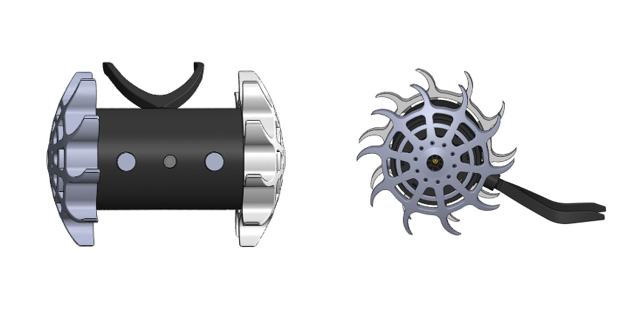
\includegraphics[width=0.5\textwidth]{Fig_First.PNG}}
\caption{HSL-Throw robot CAD view.}
\label{fig_First}
\end{figure}

\section{Existing Rescue Mobile Robot Platforms} 
The system described in this paper is designed to meet the requirements of a portable and deployable rescue robot. In recent decades, numerous mobile rescue robot platforms have been developed, emphasizing the importance of rescue and recovery systems for facilitating effective interaction between artificial intelligence and the environment. We aim to create a platform suitable for research, education, and enhancement, focusing on simplicity. In order to achieve these objectives, a robust hardware setup with diverse sensors and a modular, programmable design is essential. These features enable researchers to utilize the platform in rescue operations, training sessions, AI laboratories, and various real-world robotics applications. In this context, several robotic platforms have been specifically designed for rescue, research, and educational purposes within the field of rescue robotics. One of the most widely recognized platforms is the Recon Scout, shown in Figure~\ref{Fig_iRobotAndRecon}. While this robot is not ideally suited for high-precision rescue tasks in real environments due to its fully manual control by human operators, it remains applicable in other scenarios. Furthermore, the project presented here has developed a robotic platform that supports wireless remote communication and connectivity, allowing it to perform tasks previously challenging for most mobile robots, such as deployment in harsh conditions and waterproof operation.

\begin{figure}[htbp] 
    \centerline{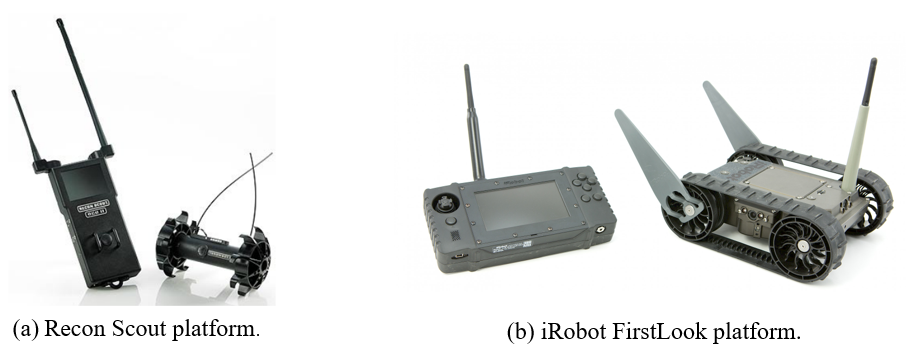
\includegraphics[width=0.5\textwidth]{Fig_iRobotAndRecon.PNG}} 
    \caption{Examples of existing rescue mobile robot platforms.} 
    \label{Fig_iRobotAndRecon} 
\end{figure}

Additionally, the IRobot FirstLook platform was reviewed (Figure~\ref{Fig_iRobotAndRecon}), capable of performing tasks on a laboratory scale. This platform can be utilized in research laboratories and technical labs, with the potential for experiences gained to be applied to industrial contexts. However, this robot is not open-source, and its cost is relatively high for students and research labs. The study emphasized the need for a compact and affordable general-purpose rescue robot for initial response. Consequently, a robust, low-cost, and portable robotic platform is currently in development, intended as a primary investigative tool in any disaster scenario. This design follows Jacoff's recommendation that the entire robotic system and necessary tools should be operable by a single operator. The robot can be deployed by being thrown or dropped from heights of up to 5 meters and is affordable enough to be considered disposable or replaceable. This ensures that rescue operations can begin without waiting for more advanced and specialized robots to arrive on the scene.

\section{System Overview}
The platform described in this paper is designed to fulfill the requirements of a portable and throwable rescue robotic system. The HSL platform consists of three main components: the mechanical structure, electronic components, and software architecture. The mechanical structure is divided into two parts: the robot's body and the movement system. The body is made of 3D-printed PLA, with a cylindrical shape, measuring 13 cm in height and 16 cm in length. The HSL's movement relies on a two-wheel robotic system. In the electronics section, the HSL consists of two main components. The first is a Raspberry Pi board with a 64-bit ARM processor, featuring Cortex-A53 architecture. It operates at a frequency of 1 GHz and runs on the Debian operating system, handling tasks related to receiving and transmitting sensor data, including images and audio, to the server. The second component is a processor based on a 32-bit ARM microcontroller with Cortex-M3 architecture, known as the STM32f103CB. It operates at a frequency of 72 MHz, has 20 KB of RAM, and 128 KB of flash memory, and runs under the FreeRTOS operating system. This unit can control and access all sensor and actuator data, such as the Inertial Measurement Unit (IMU), current, voltage, and actuator encoder. To send this information to the server, the data is first transmitted to the Raspberry Pi using the UART unit, which operates in half-duplex mode, and then the Raspberry Pi forwards it to the server based on its assigned tasks. Each input/output module can be activated or deactivated in real time by sending operational commands. This method allows the use of high-frequency sensors for specific tasks and the ability to power certain sensors/motors at a desired frequency, turn some completely off, or place them in standby mode, especially when executing complex tasks. This capability can be utilized in sensor selection algorithms and contributes to energy efficiency. The block diagram of the HSL, depicted in Figure~\ref{Fig_BlockDiagram}, can help researchers implement their algorithms more easily.

\begin{figure}[htbp] 
    \centerline{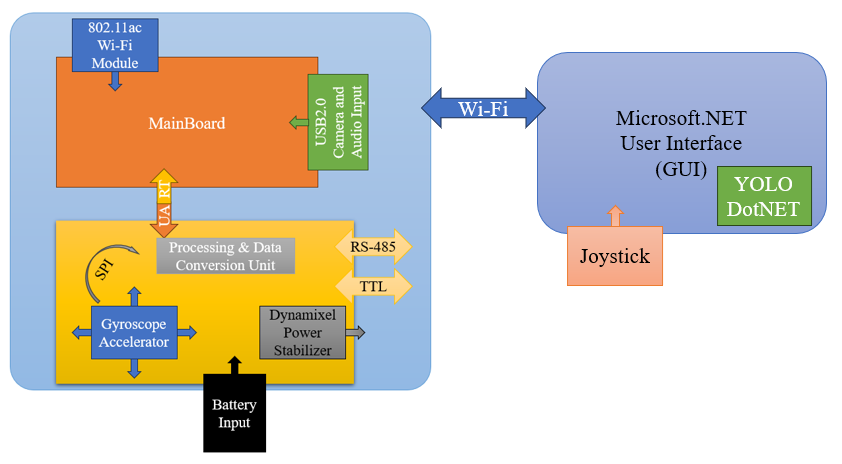
\includegraphics[width=0.5\textwidth]{BlockDiagram.PNG}} 
    \caption{Examples of existing rescue mobile robot platforms.} 
    \label{Fig_BlockDiagram}
\end{figure}

In the HSL platform, all I/O requests are handled using the FreeRTOS operating system to ensure reliable and secure information. Most primary processing, such as filtering inertial system sensor data and power management, is performed in this unit. This process is designed to collect and update all necessary information via the operating system, and if a request is made, the corresponding responses are transmitted. The management system that oversees data collection and motor update commands can reduce power consumption by controlling the reading frequency and activity of each module. Additionally, after completing all operations and sending them to the server, the user can select unique features. For instance, they can manage the YOLO algorithm's usage, choose the color format of received images, and control the activation or deactivation of audio. The robot is user-controlled via a USB PlayStation joystick. To correct for wheel deviations and navigate rough terrain, a PID controller fine-tunes the robot's movements. Furthermore, when employing the YOLO algorithm, the user can detect individuals or objects that might otherwise be missed due to disturbances.

\section{HSL-Throw Construction}
In this section, we introduce the design of the HSL robot. The implementation of the robot has been designed to be as simple as possible, and its material is plastic, which offers advantages such as low cost, appropriate weight, and good appearance. The tail connected at the outer angle of the robot serves as a handle for easier carrying and assists in throwing. Upon impact, the robot's wheels absorb a significant portion of the impact energy, protecting the internal components. Due to the hazards present in rescue environments, there is a risk of the rescue robot becoming irreversibly oriented towards the operator, as the robot stores the distance traveled in various directions during movement. In general, designers of mobile robots have divided the design problem into several subsets, such as:
\begin{itemize}
    \item Sensing
    \item Task planning and execution
    \item Motion control
\end{itemize}

We have tried to avoid these approaches and instead focus on some important factors, such as sensor and module integration, precise mechanical design, and the elimination of hardware noise for sensors, to achieve an optimized structure. To this end, instead of using a self-balancing robot motion system, a tail has been utilized to maintain balance, which also significantly aids in overcoming obstacles up to 12 centimeters in height.

\subsection{Motion System}
Dynamixel motors have been used for years in the production and applications of mobile robots. The HSL platform features a two-wheel system that allows it to move independently along each axis. An omnidirectional robot can move in a straight line from point A to point B while simultaneously rotating along the line to reach its destination with the correct orientation. Two parameters of electric motors are very important in the design and construction of wheeled robots: first, output torque, and then the no-load speed of the motor, which directly affects the acceleration and speed of the robot. The wheels designed for the HSL platform have a diameter of 15 centimeters, and the maximum adjustable speed in Dynamixel motors is 60 RPM. Considering the robot's geometry, the distance traveled and orientation of the robot can be calculated as follows:

\begin{equation}
d = \frac{(RPM \times \text{wheel diameter} \times \pi)}{60 \times t} \label{eq:distance}
\end{equation}

where \( d \) is the distance traveled.

\begin{equation}
x_{\text{new}} = x_{\text{old}} + \frac{r \times (\omega_R + \omega_L)}{2 \times \cos(\theta) \times \Delta t}
\end{equation}
\begin{equation}
y_{\text{new}} = y_{\text{old}} + \frac{r \times (\omega_R + \omega_L)}{2 \times \sin(\theta) \times \Delta t}
\end{equation}
\begin{equation}
\theta_{\text{new}} = \theta_{\text{old}} + \frac{r \times (\omega_R - \omega_L)}{L \times \Delta t}
\end{equation}

Also,
\begin{itemize}
    \item \( r \) is the radius of the wheels.
    \item \( \omega_R \) and \( \omega_L \) are the angular velocities of the right and left wheels, respectively.
    \item \( \theta \) is the orientation of the robot.
    \item \( \Delta t \) is the time increment.
    \item \( L \) is the wheelbase (the distance between the centers of the two wheels).
\end{itemize}

Finally, the characteristics of the locomotion system are shown in Table 1:

\begin{table}[htbp]
\centering
\caption{HSL Locomotion Specifications}
\begin{tabular}{|l|l|}
\hline
\textbf{Characteristics}   & \textbf{HSL Locomotion Specification} \\ \hline
Shaft encoder resolution   & 4096 [pulse/rev]                      \\ \hline
Max linear speed           & 39 cm/s                               \\ \hline
Wheel size                 & 15 cm                                 \\ \hline
No Load Speed              & 50 RPM                                \\ \hline
\end{tabular}
\label{tab:hsl_locomotion}
\end{table}


\subsection{Abbreviations and Acronyms}\label{AA}
Define abbreviations and acronyms the first time they are used in the text, 
even after they have been defined in the abstract. Abbreviations such as 
IEEE, SI, MKS, CGS, ac, dc, and rms do not have to be defined. Do not use 
abbreviations in the title or heads unless they are unavoidable.

\subsection{Units}
\begin{itemize}
\item Use either SI (MKS) or CGS as primary units. (SI units are encouraged.) English units may be used as secondary units (in parentheses). An exception would be the use of English units as identifiers in trade, such as ``3.5-inch disk drive''.
\item Avoid combining SI and CGS units, such as current in amperes and magnetic field in oersteds. This often leads to confusion because equations do not balance dimensionally. If you must use mixed units, clearly state the units for each quantity that you use in an equation.
\item Do not mix complete spellings and abbreviations of units: ``Wb/m\textsuperscript{2}'' or ``webers per square meter'', not ``webers/m\textsuperscript{2}''. Spell out units when they appear in text: ``. . . a few henries'', not ``. . . a few H''.
\item Use a zero before decimal points: ``0.25'', not ``.25''. Use ``cm\textsuperscript{3}'', not ``cc''.)
\end{itemize}

\subsection{Equations}
Number equations consecutively. To make your 
equations more compact, you may use the solidus (~/~), the exp function, or 
appropriate exponents. Italicize Roman symbols for quantities and variables, 
but not Greek symbols. Use a long dash rather than a hyphen for a minus 
sign. Punctuate equations with commas or periods when they are part of a 
sentence, as in:
\begin{equation}
a+b=\gamma\label{eq}
\end{equation}

Be sure that the 
symbols in your equation have been defined before or immediately following 
the equation. Use ``\eqref{eq}'', not ``Eq.~\eqref{eq}'' or ``equation \eqref{eq}'', except at 
the beginning of a sentence: ``Equation \eqref{eq} is . . .''

\subsection{\LaTeX-Specific Advice}

Please use ``soft'' (e.g., \verb|\eqref{Eq}|) cross references instead
of ``hard'' references (e.g., \verb|(1)|). That will make it possible
to combine sections, add equations, or change the order of figures or
citations without having to go through the file line by line.

Please don't use the \verb|{eqnarray}| equation environment. Use
\verb|{align}| or \verb|{IEEEeqnarray}| instead. The \verb|{eqnarray}|
environment leaves unsightly spaces around relation symbols.

Please note that the \verb|{subequations}| environment in {\LaTeX}
will increment the main equation counter even when there are no
equation numbers displayed. If you forget that, you might write an
article in which the equation numbers skip from (17) to (20), causing
the copy editors to wonder if you've discovered a new method of
counting.

{\BibTeX} does not work by magic. It doesn't get the bibliographic
data from thin air but from .bib files. If you use {\BibTeX} to produce a
bibliography you must send the .bib files. 

{\LaTeX} can't read your mind. If you assign the same label to a
subsubsection and a table, you might find that Table I has been cross
referenced as Table IV-B3. 

{\LaTeX} does not have precognitive abilities. If you put a
\verb|\label| command before the command that updates the counter it's
supposed to be using, the label will pick up the last counter to be
cross referenced instead. In particular, a \verb|\label| command
should not go before the caption of a figure or a table.

Do not use \verb|\nonumber| inside the \verb|{array}| environment. It
will not stop equation numbers inside \verb|{array}| (there won't be
any anyway) and it might stop a wanted equation number in the
surrounding equation.

\subsection{Some Common Mistakes}\label{SCM}
\begin{itemize}
\item The word ``data'' is plural, not singular.
\item The subscript for the permeability of vacuum $\mu_{0}$, and other common scientific constants, is zero with subscript formatting, not a lowercase letter ``o''.
\item In American English, commas, semicolons, periods, question and exclamation marks are located within quotation marks only when a complete thought or name is cited, such as a title or full quotation. When quotation marks are used, instead of a bold or italic typeface, to highlight a word or phrase, punctuation should appear outside of the quotation marks. A parenthetical phrase or statement at the end of a sentence is punctuated outside of the closing parenthesis (like this). (A parenthetical sentence is punctuated within the parentheses.)
\item A graph within a graph is an ``inset'', not an ``insert''. The word alternatively is preferred to the word ``alternately'' (unless you really mean something that alternates).
\item Do not use the word ``essentially'' to mean ``approximately'' or ``effectively''.
\item In your paper title, if the words ``that uses'' can accurately replace the word ``using'', capitalize the ``u''; if not, keep using lower-cased.
\item Be aware of the different meanings of the homophones ``affect'' and ``effect'', ``complement'' and ``compliment'', ``discreet'' and ``discrete'', ``principal'' and ``principle''.
\item Do not confuse ``imply'' and ``infer''.
\item The prefix ``non'' is not a word; it should be joined to the word it modifies, usually without a hyphen.
\item There is no period after the ``et'' in the Latin abbreviation ``et al.''.
\item The abbreviation ``i.e.'' means ``that is'', and the abbreviation ``e.g.'' means ``for example''.
\end{itemize}
An excellent style manual for science writers is \cite{b7}.

\subsection{Authors and Affiliations}\label{AAA}
\textbf{The class file is designed for, but not limited to, six authors.} A 
minimum of one author is required for all conference articles. Author names 
should be listed starting from left to right and then moving down to the 
next line. This is the author sequence that will be used in future citations 
and by indexing services. Names should not be listed in columns nor group by 
affiliation. Please keep your affiliations as succinct as possible (for 
example, do not differentiate among departments of the same organization).

\subsection{Identify the Headings}\label{ITH}
Headings, or heads, are organizational devices that guide the reader through 
your paper. There are two types: component heads and text heads.

Component heads identify the different components of your paper and are not 
topically subordinate to each other. Examples include Acknowledgments and 
References and, for these, the correct style to use is ``Heading 5''. Use 
``figure caption'' for your Figure captions, and ``table head'' for your 
table title. Run-in heads, such as ``Abstract'', will require you to apply a 
style (in this case, italic) in addition to the style provided by the drop 
down menu to differentiate the head from the text.

Text heads organize the topics on a relational, hierarchical basis. For 
example, the paper title is the primary text head because all subsequent 
material relates and elaborates on this one topic. If there are two or more 
sub-topics, the next level head (uppercase Roman numerals) should be used 
and, conversely, if there are not at least two sub-topics, then no subheads 
should be introduced.

\subsection{Figures and Tables}\label{FAT}
\paragraph{Positioning Figures and Tables} Place figures and tables at the top and 
bottom of columns. Avoid placing them in the middle of columns. Large 
figures and tables may span across both columns. Figure captions should be 
below the figures; table heads should appear above the tables. Insert 
figures and tables after they are cited in the text. Use the abbreviation 
``Fig.~\ref{fig_t1}'', even at the beginning of a sentence.

\begin{table}[htbp]
\caption{Table Type Styles}
\begin{center}
\begin{tabular}{|c|c|c|c|}
\hline
\textbf{Table}&\multicolumn{3}{|c|}{\textbf{Table Column Head}} \\
\cline{2-4} 
\textbf{Head} & \textbf{\textit{Table column subhead}}& \textbf{\textit{Subhead}}& \textbf{\textit{Subhead}} \\
\hline
copy& More table copy$^{\mathrm{a}}$& &  \\
\hline
\multicolumn{4}{l}{$^{\mathrm{a}}$Sample of a Table footnote.}
\end{tabular}
\label{tab1}
\end{center}
\end{table}

\begin{figure}[htbp]
\centerline{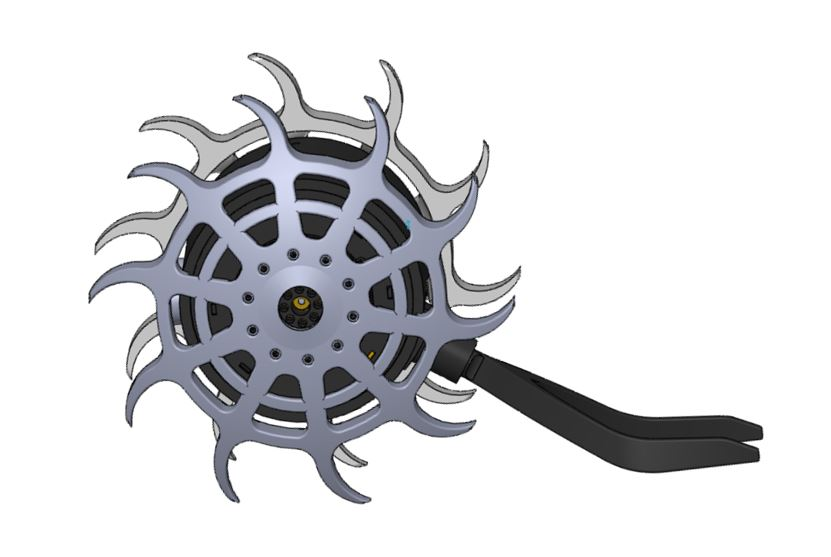
\includegraphics[width=0.5\textwidth]{Fig_T2.png}}
\caption{Example of a figure caption.}
\label{fig}
\end{figure}

Figure Labels: Use 8 point Times New Roman for Figure labels. Use words 
rather than symbols or abbreviations when writing Figure axis labels to 
avoid confusing the reader. As an example, write the quantity 
``Magnetization'', or ``Magnetization, M'', not just ``M''. If including 
units in the label, present them within parentheses. Do not label axes only 
with units. In the example, write ``Magnetization (A/m)'' or ``Magnetization 
\{A[m(1)]\}'', not just ``A/m''. Do not label axes with a ratio of 
quantities and units. For example, write ``Temperature (K)'', not 
``Temperature/K''.

\section*{Acknowledgment}

The preferred spelling of the word ``acknowledgment'' in America is without 
an ``e'' after the ``g''. Avoid the stilted expression ``one of us (R. B. 
G.) thanks $\ldots$''. Instead, try ``R. B. G. thanks$\ldots$''. Put sponsor 
acknowledgments in the unnumbered footnote on the first page.

\section*{References}

Please number citations consecutively within brackets \cite{b1}. The 
sentence punctuation follows the bracket \cite{b2}. Refer simply to the reference 
number, as in \cite{b3}---do not use ``Ref. \cite{b3}'' or ``reference \cite{b3}'' except at 
the beginning of a sentence: ``Reference \cite{b3} was the first $\ldots$''

Number footnotes separately in superscripts. Place the actual footnote at 
the bottom of the column in which it was cited. Do not put footnotes in the 
abstract or reference list. Use letters for table footnotes.

Unless there are six authors or more give all authors' names; do not use 
``et al.''. Papers that have not been published, even if they have been 
submitted for publication, should be cited as ``unpublished'' \cite{b4}. Papers 
that have been accepted for publication should be cited as ``in press'' \cite{b5}. 
Capitalize only the first word in a paper title, except for proper nouns and 
element symbols.

For papers published in translation journals, please give the English 
citation first, followed by the original foreign-language citation \cite{b6}.

\begin{thebibliography}{00}
\bibitem{b1} G. Eason, B. Noble, and I. N. Sneddon, ``On certain integrals of Lipschitz-Hankel type involving products of Bessel functions,'' Phil. Trans. Roy. Soc. London, vol. A247, pp. 529--551, April 1955.
\bibitem{b2} J. Clerk Maxwell, A Treatise on Electricity and Magnetism, 3rd ed., vol. 2. Oxford: Clarendon, 1892, pp.68--73.
\bibitem{b3} I. S. Jacobs and C. P. Bean, ``Fine particles, thin films and exchange anisotropy,'' in Magnetism, vol. III, G. T. Rado and H. Suhl, Eds. New York: Academic, 1963, pp. 271--350.
\bibitem{b4} K. Elissa, ``Title of paper if known,'' unpublished.
\bibitem{b5} R. Nicole, ``Title of paper with only first word capitalized,'' J. Name Stand. Abbrev., in press.
\bibitem{b6} Y. Yorozu, M. Hirano, K. Oka, and Y. Tagawa, ``Electron spectroscopy studies on magneto-optical media and plastic substrate interface,'' IEEE Transl. J. Magn. Japan, vol. 2, pp. 740--741, August 1987 [Digests 9th Annual Conf. Magnetics Japan, p. 301, 1982].
\bibitem{b7} M. Young, The Technical Writer's Handbook. Mill Valley, CA: University Science, 1989.
\bibitem{b8} D. P. Kingma and M. Welling, ``Auto-encoding variational Bayes,'' 2013, arXiv:1312.6114. [Online]. Available: https://arxiv.org/abs/1312.6114
\bibitem{b9} S. Liu, ``Wi-Fi Energy Detection Testbed (12MTC),'' 2023, gitHub repository. [Online]. Available: https://github.com/liustone99/Wi-Fi-Energy-Detection-Testbed-12MTC
\bibitem{b10} ``Treatment episode data set: discharges (TEDS-D): concatenated, 2006 to 2009.'' U.S. Department of Health and Human Services, Substance Abuse and Mental Health Services Administration, Office of Applied Studies, August, 2013, DOI:10.3886/ICPSR30122.v2
\bibitem{b11} K. Eves and J. Valasek, ``Adaptive control for singularly perturbed systems examples,'' Code Ocean, Aug. 2023. [Online]. Available: https://codeocean.com/capsule/4989235/tree
\end{thebibliography}

\vspace{12pt}
\color{red}
IEEE conference templates contain guidance text for composing and formatting conference papers. Please ensure that all template text is removed from your conference paper prior to submission to the conference. Failure to remove the template text from your paper may result in your paper not being published.

\end{document}
